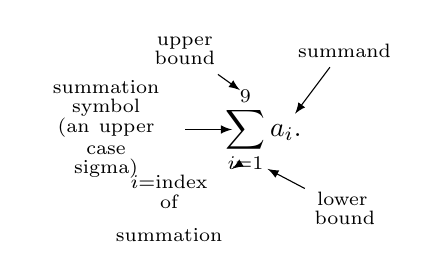
\begin{tikzpicture}[>=latex]
%\draw [thin,step=1cm] (0,0) grid  (3,3);
\draw  (1,1) node {$\displaystyle \sum_{i=1}^9 a_i$.};

\draw [{\colorone}] (-.2,0) node [text width=45pt,align=center](a) {\scriptsize \centering $i$=index \\[-5pt] of summation};
\draw [{\colorone},->] (a) -- (.6,.5);

\draw [{\colorone}] (2,0) node [text width=20pt,align=center] (b) {\scriptsize \centering lower\\[-5pt] bound};
\draw [{\colorone},->] (b) -- (1.05,.5);

\draw [{\colorone}] (0,2) node [text width=32pt,align=center] (c) {\scriptsize \centering upper\\[-5pt] bound};
\draw [{\colorone},->] (c) -- (.7,1.5);

\draw [{\colorone}] (2,2) node [text width=32pt,align=center] (d) {\scriptsize \centering summand};
\draw [{\colorone},->] (d) -- (1.4,1.2);

\draw [{\colorone}] (-1,1) node [text width=50pt,align=center] (e) {\scriptsize \centering summation \\[-1pt] symbol \\[-1pt] (an upper case\\[-5pt] sigma)};
\draw [{\colorone},->] (e) -- (.6,1);



\end{tikzpicture}
